\documentclass[ignorenonframetext, 10.5pt, aspectratio=169]{beamer}

\usepackage{kuriwaki_pream}


\title{\textbf{\Large{Sampling Simulation}}}
\author{Shiro Kuriwaki}
\date{\small\today}

\begin{document}

% TITLE ----------
\begin{frame}
\centering
\maketitle
\end{frame}



\begin{frame}
{Realistic Simulation, with full control over the sampling scheme}

\begin{itemize}
	\item Population ($N = 600,000$): CCES Data, expanded using post-stratification weights
	\begin{itemize}
	\item this is technically not a census, but it has a natural covariance structure and makes the simulation realistic
	\end{itemize}
	\item Sample ($n = 1,000$): Simple Random Sample (SRS), OR a biased sample where the propensity score for population member \(i \in \{1, ..., N\}\) is determined by:
\end{itemize}

\footnotesize
\begin{align*}
&= \text{invlogit}\left\{-4 + \begin{pmatrix}1.0\\0.8 \\0.7\\ 0.6\\ 0.5\end{pmatrix}^\top\begin{pmatrix}\text{White}_i\\\text{Black}_i\\\text{Hispanic}_i\\\text{Asian}_i\\\text{All Other}_i\\\end{pmatrix} + 
\begin{pmatrix}5.0\\4.0\\1.2\\0.5\end{pmatrix}^\top\begin{pmatrix}\text{Post-Grad}_i\\\text{4-Year}_i\\\text{Some College}_i\\\text{HS or Less}_i\end{pmatrix}  + 
\begin{pmatrix}6.0\\1.0\\ 0.4\\ 0.3\end{pmatrix}^\top\begin{pmatrix}\text{Follow News}_i\\\text{Sometimes}_i\\\text{Now and Then}_i\\\text{Hardly}_i\end{pmatrix}\right\}
\end{align*}
where White$_{i}$ for example is an indicator variable for whether respondent \(i\) is White. 


\normalsize
Then I \texttt{sample(1:N, size = n, replace = FALSE, prob =} Propensity Score$_i$\texttt{)}

\end{frame}


\begin{frame}
\centering
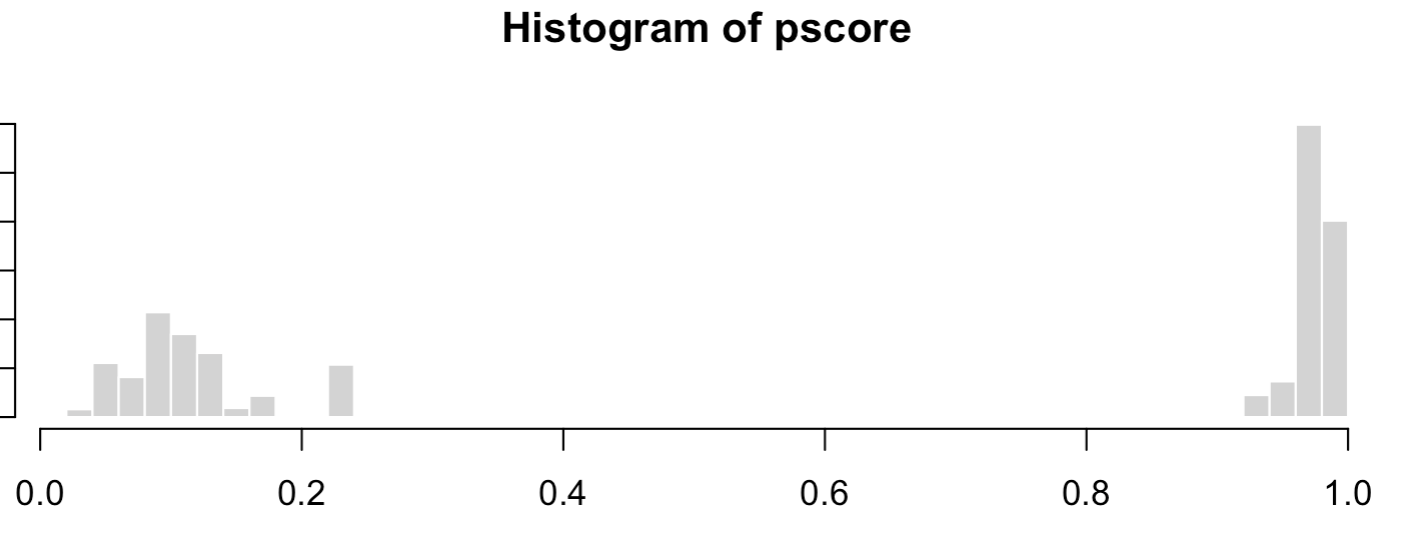
\includegraphics[width = 0.8\linewidth]{pscore.png}
\end{frame}


\begin{frame}
{Biased Sample Gives Biased Sampling Distribution}

\centering
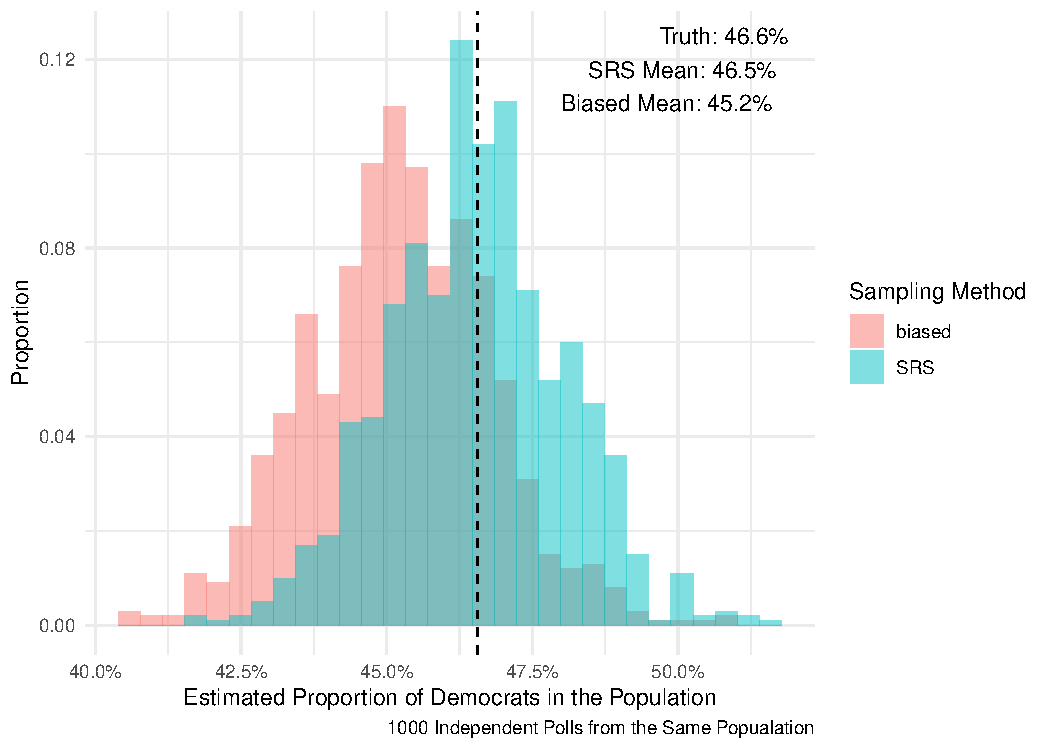
\includegraphics[width = 0.8\linewidth]{sampling.pdf}
\end{frame}


\end{document}
